\documentclass{article}

\usepackage{physics}
\usepackage{amsmath}
\usepackage{amssymb}
\usepackage{graphicx}

\begin{document}

\section{Question 1}
To begin, the angular flux is:
\begin{align*}
  \psi(x, \mu) &= \sin(\frac{x}{4})\left[1 + \left(\mu-\frac{1}{10}x\right)^2\right]
\end{align*}

\subsection{Part A}
The scalar flux is the integral with respect to angle
\begin{align*}
  \phi(x) &= \int_{-1}^1 \dd{\mu}\sin(\frac{x}{4})\left[1 + \left(\mu-\frac{1}{10}x\right)^2\right]\\
  &= \sin(\frac{x}{4}) \int_{-1}^1 \dd{\mu}\left[1 + \left(\mu-\frac{1}{10}x\right)^2\right]\\ 
  &= \sin(\frac{x}{4})\left(\frac{8}{3} + \frac{x^2}{50}\right)
\end{align*}

\begin{figure}[htbp]
  \centering
  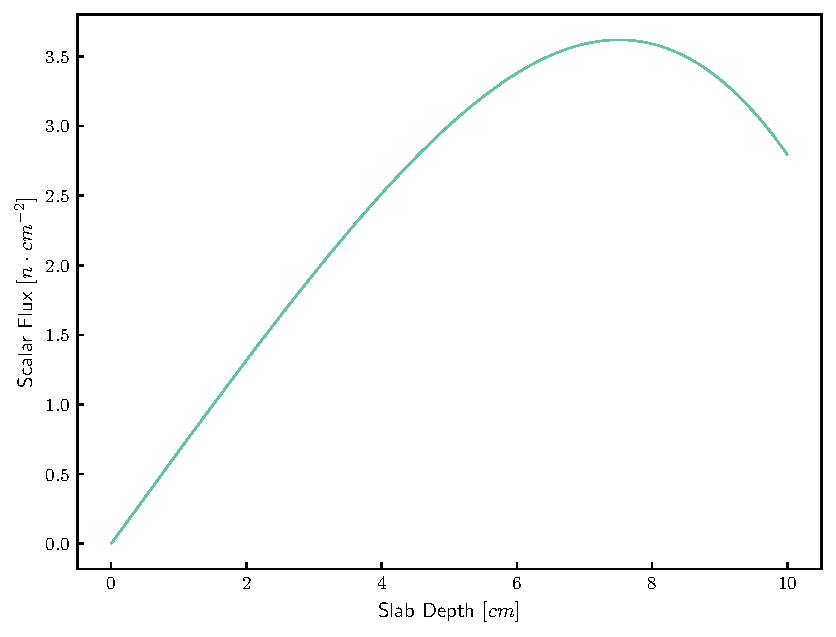
\includegraphics[width=0.5\linewidth]{hw1q1a.pdf}
\end{figure}

\subsection{Part B}
The total neutrons are found through integrating the scalar flux in space
\begin{align*}
  N &= \int_0^{10}\dd{x} \sin(\frac{x}{4})\left(\frac{8}{3} + \frac{x^2}{50}\right)\\
  &= 24.8406415566746
\end{align*}

\subsection{Part C}
First, $J^+$
\begin{align*}
  J^+(x) &= \int_0^1 \dd{\mu} \mu\psi(x, \mu)\\
  &= \int_0^1 \dd{\mu} \mu \sin(\frac{x}{4})\left[1 + \left(\mu-\frac{1}{10}x\right)^2\right]\\
  &= \sin(\frac{x}{4}) \left(\frac{x^2}{200} - \frac{x}{15} + \frac{3}{4}\right) 
\end{align*}

\begin{figure}[htbp]
  \centering
  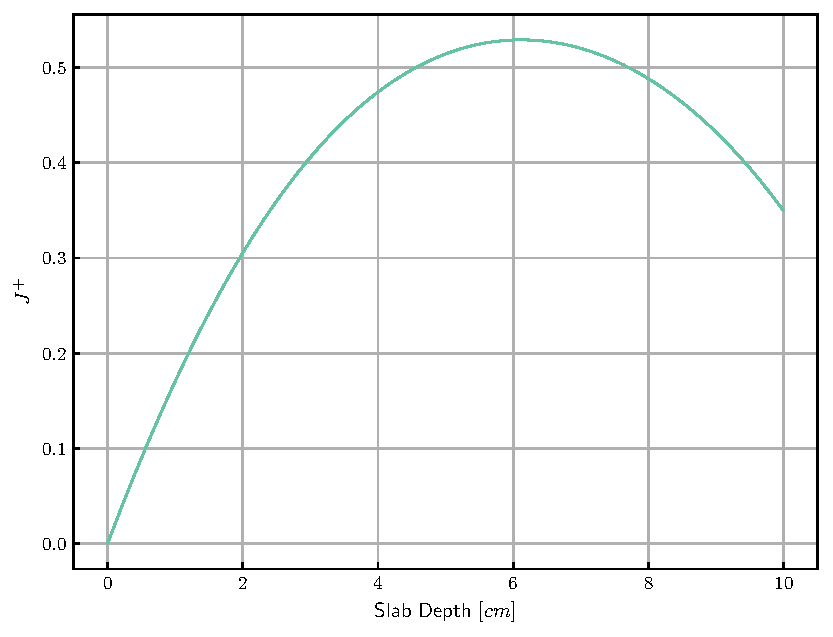
\includegraphics[width=0.5\linewidth]{hw1q1cplus.pdf}
\end{figure}
\clearpage
Then, $J^-$
\begin{align*}
  J^-(x) &= -\int_-1^0 \dd{\mu} \mu\psi(x, \mu)\\
  &= -\int_-1^0 \dd{\mu} \mu \sin(\frac{x}{4})\left[1 + \left(\mu-\frac{1}{10}x\right)^2\right]\\
  &= \sin(\frac{x}{4}) \left(\frac{x^2}{200} + \frac{x}{15} + \frac{3}{4}\right) 
\end{align*}

\begin{figure}[htbp]
  \centering
  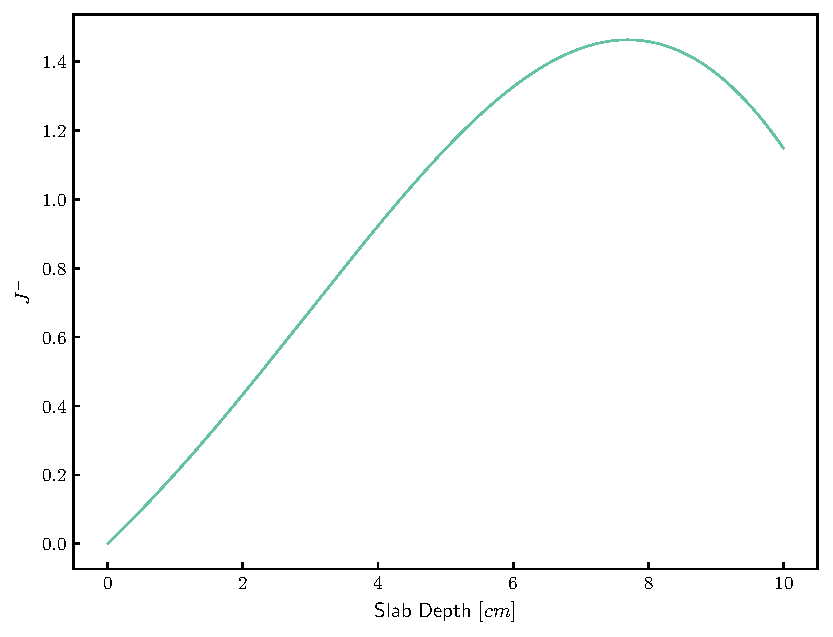
\includegraphics[width=0.5\linewidth]{hw1q1cminus.pdf}
\end{figure}
\clearpage
\subsection{Part D}
Particle current is defined via:

\begin{align*}
  J^(x) &= \int_-1^1 \dd{\mu} \mu\psi(x, \mu)\\
  &= \int_-1^1 \dd{\mu} \mu \sin(\frac{x}{4})\left[1 + \left(\mu-\frac{1}{10}x\right)^2\right]\\
  &= -\sin(\frac{x}{4}) \cdot \frac{2x}{15}
\end{align*}

\begin{figure}[htbp]
  \centering
  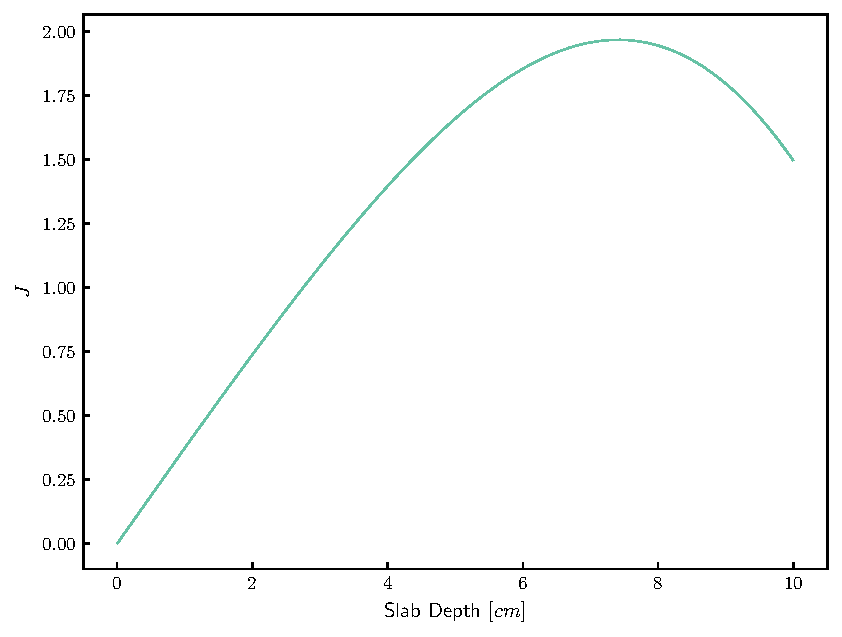
\includegraphics[width=0.5\linewidth]{hw1q1d.pdf}
\end{figure}

And the sum of the two components is:
\begin{align*}
  J^(x) &= J^+ - J^-\\
  &=  \sin(\frac{x}{4}) \left(\frac{x^2}{200} - \frac{x}{15} + \frac{3}{4}\right) -  \sin(\frac{x}{4}) \left(\frac{x^2}{200} + \frac{x}{15} + \frac{3}{4}\right)\\
  &= \sin(\frac{x}{4}) \cdot \frac{-2x}{15}
\end{align*}

\subsection{Part E}
\begin{align*}
  N_{leak} &= J^-(0) + J^+(10)\\
  &= 0 + 0.34910875072730796\\
  &= 0.34910875072730796
\end{align*}

\subsection{Part F}
\begin{align*}
  dose &= \int_0^4\dd{x}\sigma_{d,1} \phi(x) + \int_4^10\dd{x}\sigma_{d,2} \phi(x)\\
  &= 25.94597371679638 + 137.5601276932073\\
  &= 163.50610141
\end{align*}

\clearpage
\section{Question 2}
To begin, the transport equation for this question can be simplified to:
\begin{align*}
  \mu \pdv{\psi_1}{x} &= -\sigma_{t, 1}\psi_1\\
  \mu \pdv{\psi_2}{x} &= -\sigma_{t, 2}\psi_2
\end{align*}

with the following boundary conditions
\begin{align*}
  \psi_1(0) &= \psi_0\\
  \psi_1(a) &= \psi_2(a)\\
  j_1(a) &= j_2(b)\\
  \psi_2(\infty) &= 0
\end{align*}

So then the general solutions are 
\begin{align*}
  \psi_1(x) &= \psi_0e^{-\sigma_{t,1} x}\\
  \psi_2(x) &= \psi_0e^{-\sigma_{t,1} a}e^{-\sigma_{t,2} (x-a)}
\end{align*}

Then the mean free path is the first moment of the pdf:
\begin{align*}
  mfp &= \int_0^{\infty}\dd{x} x\left[\sigma_{t,1}\psi_1(x) + \sigma_{t,2}\psi_2(x)\right]\\
  &= \int_0^{a}\dd{x} x\sigma_{t,1}\psi_1(x) + \int_a^{\infty}\dd{x} x \sigma_{t,2}\psi_2(x)\\
  &= \int_0^{a}\dd{x} x\sigma_{t,1}e^{-\sigma_{t,1} x} + \int_a^{\infty}\dd{x} x \sigma_{t,2} e^{-\sigma_{t,1} a}e^{-\sigma_{t,2}(x-a)}\\
  &= \frac{e^{-a\sigma_{t,1}}\left(\frac{\sigma_{t,1}}{\sigma_{t,2}}-1\right)+1}{\sigma_{t,1}}
\end{align*}

Then, plugging in an infinite optical thickness for region 1, we obtain
\begin{align*}
  mfp &= \frac{e^{-\infty}\left(\frac{\sigma_{t,1}}{\sigma_{t,2}}-1\right)+1}{\sigma_{t,1}}\\
  &= \frac{1}{\sigma_{t,1}}
\end{align*}

Then, plugging in $\sigma_{t,2}=\sigma_{t,1}$:
\begin{align*}
  &= \frac{e^{-a\sigma_{t,1}}\left(1-1\right)+1}{\sigma_{t,1}}\\
  &= \frac{1}{\sigma_{t,1}}
\end{align*}

\clearpage
\section{Question 3}


\clearpage
\newcommand{\psig}{\psi^{\gamma}}
\newcommand{\psin}{\psi^{n}}
\newcommand{\phase}{\left(\vec{r}, \hat{\Omega}, E, t\right)}
\newcommand{\renergy}{\left(\vec{r}, E\right)}
\newcommand{\double}{\left(\vec{r}, \hat{\Omega}' \rightarrow \hat{\Omega}, E'\rightarrow E\right)}
\newcommand{\psid}{\left(\vec{r}, \hat{\Omega}', E', t\right)}
\section{Question 4}
\subsection{Part A}
\begin{multline*}
  \frac{1}{c} \pdv{\psig\phase}{t}
  + \hat{\Omega}\cdot\grad\psig\phase
  + \sigma^{\gamma}_t\psig
  \\
  =
  \int_{4\pi}\int_0^{\infty}\dd{E'}\dd{\hat{\Omega}'}\sigma_s^{\gamma}\double \psig\psid
  \\+ \frac{\delta(E - m_ec^2)}{2\pi}\int_0^{\infty}\sigma_p^{\gamma}\renergy\psi\phase
  + q^{\gamma}\phase
\end{multline*}

\subsection{Part B}
\begin{multline*}
  \frac{1}{c} \pdv{\psig\phase}{t}
  + \hat{\Omega}\cdot\grad\psig\phase
  + \sigma^{\gamma}_t\psig
  \\
  =
  \int_{4\pi}\int_0^{\infty}\dd{E'}\dd{\hat{\Omega}'}\sigma_s^{\gamma}\double \psin\psid
  \\+ \frac{\delta(E - m_ec^2)}{2\pi}\int_0^{\infty}\sigma_p^{\gamma}\renergy\psi\phase
  \\+ \frac{\chi^{\gamma}(\vec{r}, E'\rightarrow E)}{4\pi}\int_0^{\infty}\dd{E'}\nu^{\gamma}\renergy\sigma_t^n\renergy\psin\left(\vec{r}, \Omega, E', t\right)
  + q^{\gamma}\phase
\end{multline*}

\begin{multline*}
  \frac{1}{v^n(E)} \pdv{\psin\phase}{t}
  + \hat{\Omega}\cdot\grad\psin\phase
  + \sigma^{n}_t\psin
  \\
  =
  \int_{4\pi}\int_0^{\infty}\dd{E'}\dd{\hat{\Omega}'}\sigma_{\gamma,n}^{\gamma}\double \psig\psid
  \\ + \int_{4\pi}\int_0^{\infty}\dd{E'}\dd{\hat{\Omega}'}\sigma_s^{n}\double \psin\psid
  \\+ \frac{\chi^{n}(\vec{r}, E'\rightarrow E)}{4\pi}\int_0^{\infty}\dd{E'}\nu^{n}\renergy\sigma_f^n\renergy\psin\left(\vec{r}, \Omega, E', t\right)
  + q^n\phase
\end{multline*}

\end{document}